\begin{document}
\onehalfspacing
\begin{center}
{\Large\bfseries When interval coverage hides the direction of maintenance-trigger errors: a sensor-degradation stress test of remaining-useful-life prediction intervals\par}
\vspace{0.6em}
\ifanon
{\small Original Research Article --- anonymised manuscript for review\par}
\else
{\normalsize Yi Wang\par}
{\small College of Engineering, Lishui University, Lishui 323000, Zhejiang, China\par}
{\small Corresponding author: Yi Wang, \texttt{jefflsxy@lsu.edu.cn}\par}
\fi
\end{center}
\vspace{0.4em}
\begin{abstract}\noindent
Maintenance rules often act when a lower prediction bound on remaining useful life (RUL) reaches a lead time, while the bound itself is judged by its coverage. We ask whether coverage, including the one-sided coverage that such a rule relies on, reveals which maintenance error a degraded sensor causes. On C-MAPSS (four sub-datasets, LSTM and Transformer backbones, five interval mechanisms, disjoint fitting, validation and calibration engines), sensor drift, offsets and channel subsets were applied to the last window of each test engine and to whole test trajectories, with magnitudes expressed in within-operating-condition standard deviations (SD). A drift of $+1$ to $+2$ SD sent \RVPremOne\% and \RVPremTwo\% of evaluated engines into premature maintenance at a 20-cycle lead time while the one-sided coverage of the lower bound rose to \RVCovTwo; the mirror-image drift left \RVLateNegCondTwo\% of the engines that needed maintenance untriggered while central coverage fell to a similar level. The side of the error followed whether the shift moved inputs along or against the direction the model reads as degradation; one of \RVChanN{} single-channel ramps reached \RVChanMax\% premature triggers, and the pattern held at three bound levels, three tolerance bands and three lead times. Expressing perturbations as a share of the training range, as is common, made shifts on six-condition data about \RVRatioFactor{} times larger in SD units than on single-condition data and produced an apparent dataset contrast that disappears in SD units. Interval evaluations meant for maintenance should therefore report both trigger errors and scale perturbations within operating regimes. Results are simulated and inference-only.
\end{abstract}
\noindent\textbf{Keywords:} remaining useful life; prediction intervals; conformal prediction; sensor drift; maintenance decision; C-MAPSS
\bigskip

\section{Introduction}
A prediction interval on remaining useful life (RUL) becomes an engineering commitment when a maintenance rule consumes it. A planner who triggers work whenever a one-sided lower bound falls to or below a lead time of twenty cycles relies on that bound in two directions: it must not be so low that equipment far from needing attention is pulled early, and not so high that equipment that needs attention stays in service. The bound is usually summarised by coverage and width on clean inputs. Coverage counts how often the truth lies inside the interval; it does not say which of the two maintenance errors a failure of the interval produces.

The nearest prior work comes from three directions (Supplement S8 compares fourteen studies). Decision-oriented evaluation of prognostics has been developed on clean inputs: Kamariotis et al.\cite{kamariotis2024} define a metric from the long-run maintenance cost of a policy relative to perfect prognostics, and Mitici et al.\cite{mitici2023}, de Pater et al.\cite{depater2022} and Lee and Mitici\cite{lee2022} feed probabilistic RUL into replacement, alarm and reinforcement-learning policies; Mitici et al.\ find the optimal replacement close to the 99\% lower bound, which is the rule family studied here. Uncertainty-quantification benchmarks compare heteroscedastic networks, MC Dropout, deep ensembles and conformal methods by calibration and sharpness, including on out-of-distribution units,\cite{basora2025,piao2025,xu2026,javanmardi2022} but without a maintenance rule; Basora et al.\ conclude that no method wins everywhere. Sensor degradation has been treated either as a joint stochastic process with system degradation\cite{hachem2024} or as missing or malfunctioning channels for point prediction.\cite{xu2023,tang2026} None of these studies asks whether the interval metrics in use would reveal the direction of the maintenance error when sensors degrade, and the decision studies, which do count errors, use clean inputs.

This paper addresses that question with a controlled stress test on C-MAPSS. Intervals come from five mechanisms on two backbones for the four sub-datasets, under an engine-level protocol with disjoint fitting, validation and calibration engines. We perturb the sensor channels of each test engine with ramps, offsets and channel subsets whose sizes are expressed in within-operating-condition standard deviations, apply a one-sided lower-bound rule, and count separately the engines that needed maintenance but were not triggered and the engines triggered although far from needing it. Three questions are asked. (Q1) Do central and one-sided coverage, and the share of out-of-range inputs, reveal the direction and size of the trigger errors? (Q2) What sets the direction: the sign of the shift, its alignment with the degradation signature, the number of channels, its temporal form? (Q3) Are the answers stable to the bound level, the tolerance that defines a premature trigger, the lead time and the calibration unit, and how much does the choice of a perturbation scale change them?

The contributions are bounded by the conditions stated in later sections. First, evidence that the one-sided coverage of a lower bound, the guarantee that a lower-bound maintenance rule relies on, is blind to the premature side: it approaches 1.00 exactly when most engines far from failure are triggered, and it falls only when needed maintenance is missed. Second, evidence that the side of the error follows whether the sensor shift moves the input along or against the direction the model reads as degradation, at the level of all channels, of channel subsets and of single channels, for ramps within a window and for drifts that accumulate along a trajectory, and that the pattern survives changes of bound level, tolerance band, lead time and calibration unit. Third, a methodological observation for robustness studies: perturbation sizes set as a share of the training range are not comparable across operating regimes, and on C-MAPSS they create an apparent dataset contrast that disappears when sizes are expressed within regimes. The study is empirical and inference-only; it proposes no architecture, drift detector or maintenance policy, and its data are simulated.

\section{Evaluation and maintenance-decision framework}\label{sec:framework}
\subsection{Data, evaluation unit and labels}
C-MAPSS (FD001--FD004)\cite{saxena2008} provides run-to-failure training trajectories and test trajectories truncated before failure, with the terminal RUL supplied separately. FD001 and FD003 have one operating condition and 14 sensor channels; FD002 and FD004 have six conditions, 15 sensor channels and three operating-setting channels. The model input is a window of 30 cycles. Models predict $\min(\mathrm{RUL}_{t+1},125)$, the clipped RUL at the cycle after the window, and test engines are scored against $\min(\mathrm{RUL}-1,125)$ from the official terminal label, so training, calibration, checkpoint selection and testing share one target instant; scoring against the current-cycle label changes the headline decision rates by at most \JLabelHeadline{} points. The main evaluation unit is the last window of each test engine; engines with fewer than 30 recorded cycles are excluded, leaving \JEvalEng{} evaluated engines for FD001--FD004 (\JFileEng{} in the files). A trajectory analysis (Section~\ref{sec:traj}) uses every window of each test engine.

\begin{figure}[!t]
\centering
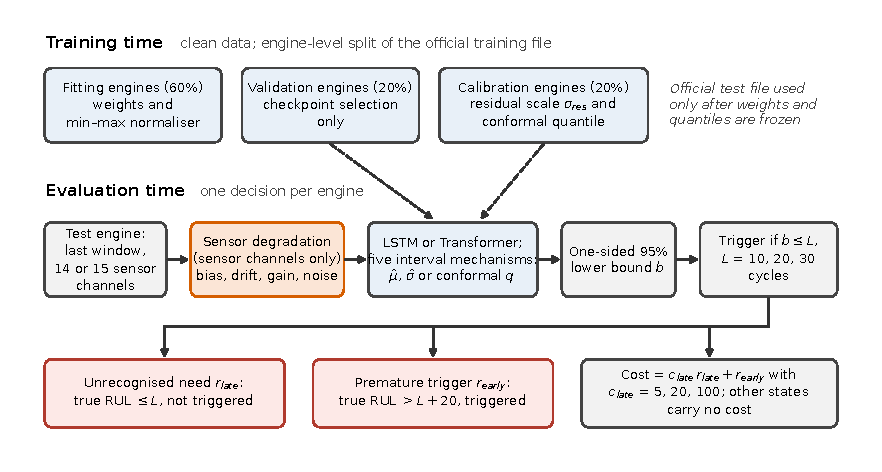
\includegraphics[width=\textwidth]{figures/fig1.pdf}
\caption{Evaluation protocol from clean training-time engine partitions to a maintenance decision per test engine. The scheme describes the stress test performed here; it is not a deployed monitoring system.}
\label{fig:flow}
\end{figure}

\subsection{Models, calibration and leakage control}
The LSTM has two layers of 64 units with dropout 0.2; the Transformer applies two encoder layers ($d=64$, four heads) with average pooling. Both were trained with Adam for 150 epochs with hyperparameters fixed before the protocol was adopted. Five interval mechanisms are built on them: a fixed-variance head (MSE training, one global residual scale), a heteroscedastic Gaussian head (mean and log-scale outputs\cite{nix1994}), MC Dropout ($T=50$, predictive variance including the residual term\cite{gal2016,kendall2017}), a deep ensemble (the five heteroscedastic seeds combined by moment matching\cite{lakshminarayanan2017}) and split conformal prediction with a normalised score (CP-norm\cite{barber2023}).

Each of five seeds draws its own engine-level partition of the official training file (Figure~\ref{fig:flow}): 60\% of engines fit the weights and the min--max normaliser, 20\% select the checkpoint, and 20\% calibrate the conformal quantile and, for the fixed-variance and MC Dropout mechanisms, the residual scale. The official test file is used once, after all quantities are frozen. The protocol replaces an earlier pipeline in which the checkpoint had been selected on the test set. A controlled $2\times2$ retraining with the fitting engines held fixed (Supplement S1) isolates the two choices. On FD001, test-set checkpoint selection lowers RMSE by 1.94 cycles on average over the two normaliser scopes (12.6\% of the validation-selected value) and, with the normaliser scope held fixed, lowers the NASA score by 48.7\% (552.2 to 283.1) and 51.9\% (558.4 to 268.4); the normaliser scope moves RMSE by at most \NNormAbsMaxRMSE{} cycles. The intervals analysed here are therefore not products of test-set selection; the models are not state of the art.

\emph{Calibration unit.} The conformal quantile and the residual scales are computed from all overlapping windows of the calibration engines (\RVCalWin{} windows from \RVCalEng{} engines per partition), whereas the test unit is one truncated terminal window per engine. Windows of one engine are dependent, and their label distribution differs from that of truncated terminal windows, so exchangeability between calibration and test units, on which the conformal guarantee rests,\cite{barber2023} is not given by the engine-disjoint split alone. Three alternative calibration units are therefore compared (Section~\ref{sec:clean}): an engine-weighted quantile (each calibration engine weighted equally), a label-matched quantile (calibration windows re-weighted to the histogram of clipped test labels, a diagnostic that uses the test label distribution but no engine-level test label), and one randomly drawn window per calibration engine (500 draws).

\emph{Predicted-mean processing.} The stress-test code leaves the heteroscedastic mean (also used by CP-norm) and ensemble members unclipped and clips the other means; the clean baseline is recomputed through the same code path (Supplement S2). Clipping changes none of the heteroscedastic or CP-norm trigger rates in \JClipRateN{} stored cells and the ensemble rates by at most \JClipRateMaxEns{} points.

\subsection{Sensor degradation and its scale}\label{sec:pert}
Perturbations act on the raw readings of the sensor channels before normalisation, without retraining; operating-setting channels are never perturbed. The size of a perturbation needs a reference. A share of each channel's range over the training file is a common choice, but on the six-condition sub-datasets that range spans six operating regimes: 5\% of it equals a median of \RVRatioSix{} within-condition standard deviations (\RVRatioSixRange{} across channels), against \RVRatioSingle{} on the single-condition sub-datasets. We therefore express sizes in units of the within-condition standard deviation of each channel (SD; condition clusters by $k$-means on the settings, mean of the per-condition SDs over the training file). The range-based families of the earlier analysis (noise, bias, drift and gain at 0.1--5\% of range) are kept in Supplements S3--S5 for comparability.

\emph{Ramp} adds a linear ramp from zero to $\pm k$ SD over the 30 steps of the final window, $k\in\{0.5,1,2,4\}$, on every sensor channel with one sign. \emph{Aligned} and \emph{anti-aligned} ramps give each channel the sign of its own degradation trend or the opposite sign; the trend sign is that of the Spearman correlation between the condition-centred reading and $-$RUL on the fitting engines (it is negative for P30, phi, W31 and W32 and positive for the other channels on every sub-dataset). \emph{Offset} adds a constant $\pm k$ SD with a random sign per channel (five realisations). \emph{Channel subsets} apply a $+2$ SD ramp to one or three randomly chosen sensor channels (ten draws each), and every channel is also ramped singly by $\pm2$ SD. \emph{Trajectory drift} adds $0.02$ SD per cycle from the first recorded cycle of each test trajectory (2 SD after 100 cycles), with all channels positive or degradation-aligned, so that the shift accumulates in physical time rather than being re-zeroed in every window. The share of out-of-range inputs, $f_{\mathrm{oob}}$, is the fraction of normalised sensor inputs of the evaluated windows outside $[-1,1]$.

\subsection{Maintenance rule and error accounting}
For each mechanism the rule computes a one-sided lower bound $b$ at level $1-\alpha$, with $\alpha=0.05$ in the main analysis and $\alpha\in\{0.10,0.01\}$ as sensitivity. For the Gaussian mechanisms $b=\hat\mu-z_{1-\alpha}\hat\sigma$; at $\alpha=0.05$ this is the lower limit of their central 90\% interval, whose coverage is reported as PICP. For CP-norm, $b=\hat\mu-q\hat\sigma$ with $q$ the conformal quantile of the \emph{signed} normalised score at level $1-\alpha$. Maintenance is triggered when $b\le L$, $L\in\{10,20,30\}$ cycles. The \emph{one-sided coverage} is the share of evaluated engines with true RUL $y\ge b$, the property the rule relies on.

An \emph{unrecognised maintenance need} is $y\le L$ with no trigger; a \emph{premature trigger} is a trigger with $y>L+\tau$, with tolerance band $\tau=20$ cycles in the main analysis and $\tau\in\{10,40\}$ as sensitivity. Both rates use all evaluated engines as denominator; the conditional unrecognised rate uses the engines with $y\le L$ (\RVAtRisk\% of evaluated engines at $L=20$). Because only engines with $y>L+\tau$ can be triggered prematurely (\RVFar\% at $L=20$, $\tau=20$), that share is the ceiling of the premature rate. Costs $c_{\mathrm{late}}r_{\mathrm{late}}+r_{\mathrm{early}}$ with $c_{\mathrm{late}}\in\{5,20,100\}$ are used only to ask how a mechanism ranking depends on the cost ratio; they are a binary loss, not a maintenance-cost model.

\subsection{Statistical units and uncertainty}
The resampling unit is the engine. Each rate is the mean over engines of the per-engine mean over the five models (and over realisations or channel draws where these exist). Intervals are percentile intervals from 2000 bootstrap resamples of engines, conditional on the five trained models, whose initialisation and partition variability are confounded; model-to-model ranges are reported separately. When no evaluated engine shows an event in any model, the percentile interval is degenerate, $[0,0]$, and says nothing about the population rate; we then report the exact one-sided 95\% upper bound for an engine-level event probability with zero events, \RVZeroUpperOne\% for 100 engines and \RVZeroUpperTwo--\RVZeroUpperFour\% for the six-condition test sets. All analyses are inference on released checkpoints, run once after the protocol was fixed; they are exploratory and not pre-registered. Re-running the earlier decision analysis with the new code reproduces the released decision rates of the deterministic mechanisms within 0.08 points and the released conformal quantiles within \RVCPqDiff.

\section{Results}\label{sec:results}
\subsection{Clean baseline and calibration unit}\label{sec:clean}
On clean inputs the central 90\% coverage lies in \JCleanCovAll{} across mechanisms, backbones and sub-datasets (Table~\ref{tab:clean}). The one-sided coverage of the 95\% lower bound is lower than nominal for the single-model mechanisms: \RVCovOneNLL\% for the heteroscedastic head and \RVCovOneCP\% for CP-norm, \RVCovOneFix\% for the fixed-variance head, \RVCovOneMC\% for MC Dropout and \RVCovOneEns\% for the ensemble (Supplement S9). Its engine-bootstrap interval lies wholly below 0.95 in \RVCovOneNLLBelow{} of 8 cells for the heteroscedastic head and \RVCovOneCPBelow{} for CP-norm. A central coverage near 90\% therefore does not certify the one-sided bound that the rule uses.

The calibration unit explains part of the conformal shortfall. Weighting calibration engines equally raises the conformal quantile from \RVQAll{} to \RVQEW{} and the one-sided coverage of CP-norm to \RVCovOneEW\%; matching the label histogram gives \RVCovOneLM\%, and one window per engine gives \RVCovOneOPE\% on average, with quantiles of \RVQOPE{} because the finite-sample correction for about twenty engines selects one of the largest scores. These alternatives change clean premature rates of CP-norm by \RVCalCleanPremShift{} points and, under the range-scale perturbations of the earlier analysis, its premature rates on the six-condition sub-datasets by at most \RVCalDriftShiftSix{} points and its unrecognised rates by \RVCalLateShift{} points. The calibration unit thus matters for the clean guarantee but does not drive the stress-test findings below.

\begin{table}[!t]
\caption{Clean-input interval benchmark under fair calibration, recomputed with the stress-test processing of the predicted mean, terminal unit, mean of five seeds. Coverage is the range of the central 90\% PICP over the four sub-datasets; MPIW (cycles) and interval score IS (lower is better) are means over the four sub-datasets. One-sided coverage of the 95\% lower bound is in Supplement S9.}
\label{tab:clean}
\centering\small
\begin{tabular}{lccc|ccc}
\toprule
 & \multicolumn{3}{c|}{LSTM} & \multicolumn{3}{c}{Transformer} \\
Mechanism & PICP & MPIW & IS & PICP & MPIW & IS \\
\midrule
Fixed variance & 0.87--0.91 & 54 & 76.3 & 0.84--0.92 & 51 & 75.0 \\
Heteroscedastic & 0.86--0.91 & 47 & 68.4 & 0.86--0.89 & 46 & 69.6 \\
MC Dropout & 0.89--0.93 & 56 & 75.5 & 0.88--0.92 & 53 & 69.5 \\
Deep ensemble & 0.91--0.96 & 50 & 63.3 & 0.91--0.93 & 49 & 63.2 \\
Split-CP (norm) & 0.88--0.93 & 51 & 68.2 & 0.86--0.91 & 48 & 69.8 \\
\bottomrule
\end{tabular}
\end{table}

\subsection{Coverage does not show the side of the error}\label{sec:side}
Figure~\ref{fig:side} and Table~\ref{tab:sd} give the heteroscedastic head at $L=20$. A positive ramp on all sensor channels lowers the predicted mean and moves engines far from failure into maintenance: \RVPremHalf\% of evaluated engines at $+0.5$ SD, \RVPremOne\% at $+1$ SD and \RVPremTwo\% at $+2$ SD, close to the ceiling of \RVFar\% set by the engines that can be triggered prematurely. No unrecognised need occurs (at most \RVUnrecPosTwo\% of engines; with no event in any engine and model, the population rate is below \RVZeroUpperTwo--\RVZeroUpperFour\% on the six-condition data by the exact bound of Section~\ref{sec:framework}). The mirror-image ramp raises the mean and produces the opposite error: unrecognised needs in \RVLateNegTwo\% of evaluated engines at $-2$ SD, that is \RVLateNegCondTwo\% of the engines that needed maintenance, and premature triggers in at most \RVPremNegTwo\%. The same split holds for every mechanism: premature rates at $+2$ SD of \RVPremTwoAllMech\% and unrecognised rates at $-2$ SD of \RVLateTwoAllMech\% across the five mechanisms, so the choice of mechanism does not remove the error. Engine-bootstrap half-widths are at most \RVPremTwoHalfCI{} points.

The interval metrics respond very differently to the two sides. The central PICP falls on both sides (\RVPicpTwo{} at $+2$ SD, \RVPicpNegTwo{} at $-2$ SD) and therefore does not say which way the rule fails. The one-sided coverage of the lower bound, the property the rule relies on, falls to \RVCovNegTwo{} under the negative ramp but \emph{rises} to \RVCovTwo{} under the positive ramp, exactly where premature triggers are most frequent: a bound that is far too low always covers the truth from below. The share of out-of-range inputs stays at or below \RVFoobTwo\% for all these shifts, so it flags neither side. Random-sign offsets of $\pm2$ SD fall in between, with premature triggers in \RVPremBiasTwo\% and unrecognised needs in \RVLateBiasTwo\% of engines at one-sided coverage of \RVCovBiasTwo.

\begin{figure}[!t]
\centering
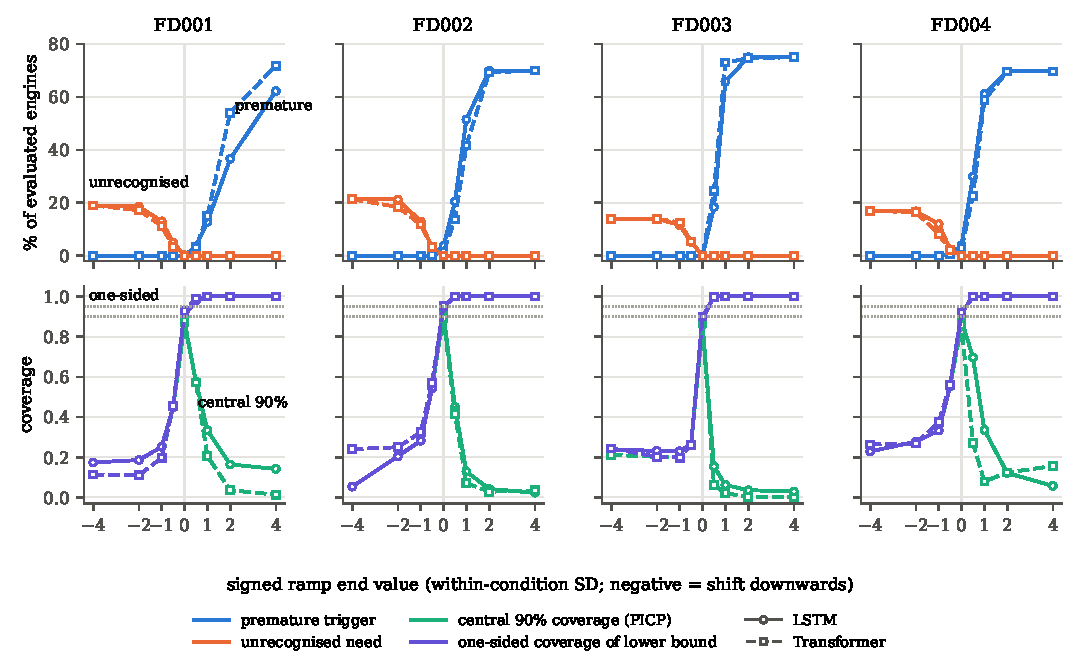
\includegraphics[width=\textwidth]{figures/fig2.pdf}
\caption{Trigger errors (top) and coverage (bottom) of the heteroscedastic head against the signed end value of a ramp on all sensor channels of the final window, in within-condition standard deviations; $L=20$, one-sided 95\% bound, mean of five models. Dotted lines mark 0.90 and 0.95. Negative values shift readings downwards. The premature rate is bounded by the share of engines with true RUL above 40 cycles (\RVFar\%).}
\label{fig:side}
\end{figure}

\begin{table}[!t]
\caption{Stress test in within-condition SD units, heteroscedastic head, $L=20$, one-sided 95\% bound. PICP: central 90\% coverage; one-sided: share of engines with true RUL above the lower bound; $f_{\mathrm{oob}}$: \% of normalised sensor inputs outside $[-1,1]$. Rates are \% of evaluated engines with engine-bootstrap 95\% intervals (2000 resamples, conditional on the five models). An interval of $[0.0, 0.0]$ means that no engine showed the event; see Section~\ref{sec:framework} for the exact upper bound. All mechanisms, lead times and shift sizes: supplementary CSV files.}
\label{tab:sd}
\centering\scriptsize
\begin{tabular}{llccccccc}\toprule
 & & \multicolumn{3}{c}{Coverage} & \multicolumn{2}{c}{Premature (\%)} & \multicolumn{2}{c}{Unrecognised (\%)} \\
\cmidrule(lr){3-5}\cmidrule(lr){6-7}\cmidrule(lr){8-9}
Cell & Shift & PICP & One-sided & $f_{\mathrm{oob}}$ & rate & [95\% CI] & rate & [95\% CI] \\ \midrule
LSTM FD001 & none & 0.86 & 0.90 & 0.0 & 0 & [0, 0] & 0.2 & [0.0, 0.6] \\
 & $+2$ SD ramp & 0.16 & 1.00 & 1.1 & 37 & [28, 45] & 0.0 & [0.0, 0.0] \\
 & $-2$ SD ramp & 0.19 & 0.19 & 4.8 & 0 & [0, 0] & 18.6 & [11.6, 26.2] \\
 & $\pm2$ SD offset & 0.32 & 0.63 & 13.4 & 8 & [6, 9] & 5.2 & [2.8, 7.9] \\
\addlinespace[2pt]
LSTM FD002 & none & 0.91 & 0.95 & 0.0 & 4 & [2, 6] & 0.0 & [0.0, 0.0] \\
 & $+2$ SD ramp & 0.04 & 1.00 & 1.5 & 70 & [64, 75] & 0.0 & [0.0, 0.0] \\
 & $-2$ SD ramp & 0.20 & 0.20 & 1.3 & 0 & [0, 0] & 21.3 & [16.6, 26.2] \\
 & $\pm2$ SD offset & 0.33 & 0.76 & 2.5 & 21 & [19, 24] & 3.9 & [2.9, 5.0] \\
\addlinespace[2pt]
LSTM FD003 & none & 0.86 & 0.89 & 0.0 & 0 & [0, 0] & 0.0 & [0.0, 0.0] \\
 & $+2$ SD ramp & 0.04 & 1.00 & 1.7 & 75 & [67, 83] & 0.0 & [0.0, 0.0] \\
 & $-2$ SD ramp & 0.23 & 0.23 & 6.7 & 0 & [0, 0] & 14.0 & [8.0, 21.0] \\
 & $\pm2$ SD offset & 0.37 & 0.69 & 17.4 & 17 & [14, 20] & 2.0 & [0.7, 3.4] \\
\addlinespace[2pt]
LSTM FD004 & none & 0.88 & 0.92 & 0.4 & 4 & [2, 6] & 0.1 & [0.0, 0.3] \\
 & $+2$ SD ramp & 0.12 & 1.00 & 0.9 & 70 & [63, 76] & 0.0 & [0.0, 0.0] \\
 & $-2$ SD ramp & 0.28 & 0.28 & 1.8 & 0 & [0, 0] & 16.8 & [11.8, 21.7] \\
 & $\pm2$ SD offset & 0.46 & 0.85 & 3.3 & 29 & [26, 33] & 2.3 & [1.6, 3.2] \\
\addlinespace[2pt]
Transformer FD001 & none & 0.88 & 0.93 & 0.0 & 0 & [0, 0] & 0.0 & [0.0, 0.0] \\
 & $+2$ SD ramp & 0.04 & 1.00 & 1.1 & 54 & [46, 62] & 0.0 & [0.0, 0.0] \\
 & $-2$ SD ramp & 0.11 & 0.11 & 4.8 & 0 & [0, 0] & 17.2 & [10.2, 25.0] \\
 & $\pm2$ SD offset & 0.42 & 0.65 & 13.4 & 6 & [5, 8] & 5.5 & [3.0, 8.5] \\
\addlinespace[2pt]
Transformer FD002 & none & 0.89 & 0.95 & 0.0 & 2 & [0, 3] & 0.1 & [0.0, 0.2] \\
 & $+2$ SD ramp & 0.03 & 1.00 & 1.5 & 69 & [63, 75] & 0.0 & [0.0, 0.0] \\
 & $-2$ SD ramp & 0.25 & 0.25 & 1.3 & 0 & [0, 0] & 18.4 & [14.2, 22.8] \\
 & $\pm2$ SD offset & 0.28 & 0.77 & 2.5 & 22 & [20, 24] & 5.1 & [3.8, 6.5] \\
\addlinespace[2pt]
Transformer FD003 & none & 0.87 & 0.90 & 0.0 & 0 & [0, 0] & 0.0 & [0.0, 0.0] \\
 & $+2$ SD ramp & 0.00 & 1.00 & 1.7 & 75 & [66, 83] & 0.0 & [0.0, 0.0] \\
 & $-2$ SD ramp & 0.20 & 0.20 & 6.7 & 0 & [0, 0] & 14.0 & [7.0, 21.0] \\
 & $\pm2$ SD offset & 0.41 & 0.82 & 17.4 & 19 & [16, 23] & 0.2 & [0.0, 0.3] \\
\addlinespace[2pt]
Transformer FD004 & none & 0.86 & 0.92 & 0.4 & 3 & [1, 5] & 0.0 & [0.0, 0.0] \\
 & $+2$ SD ramp & 0.12 & 1.00 & 0.9 & 70 & [64, 76] & 0.0 & [0.0, 0.0] \\
 & $-2$ SD ramp & 0.27 & 0.27 & 1.8 & 0 & [0, 0] & 16.5 & [12.1, 21.4] \\
 & $\pm2$ SD offset & 0.27 & 0.85 & 3.3 & 25 & [22, 28] & 2.0 & [1.4, 2.8] \\
\bottomrule\end{tabular}

\end{table}

\subsection{Alignment with the degradation signature sets the side}\label{sec:align}
Giving each channel the sign of its own degradation trend produces premature triggers in \RVPremAligned\% of evaluated engines at 2 SD, at the ceiling on every sub-dataset; the opposite signs produce unrecognised needs in \RVLateAnti\% (Supplement S10). The all-positive ramp behaves almost like the aligned ramp because eleven of the fourteen or fifteen channels rise towards failure. The error therefore follows whether the shift mimics or masks the degradation signature the model has learned, not the sign of the readings as such.

Full-channel coherence is not needed. A $+2$ SD ramp on one random channel gives a median of \RVKOneMed\% premature triggers over the ten draws per cell, but up to \RVKOneMax\%; three channels give medians of \RVKThreeMed\% and up to \RVKThreeMax\%. Ramping every channel singly (Figure~\ref{fig:chan}), \RVChanGtTen{} of the \RVChanN{} channel--cell combinations exceed 10\% premature triggers, with a maximum of \RVChanMax\% (\RVChanMaxSixCond\% on six-condition data, mainly from Ps30, NRc and T50, and \RVChanMaxSingleCond\% on single-condition data). Reversing the sign of the ramp moves the error to the other side in \RVChanFlip{} of the \RVChanMaterial{} combinations with a material effect; the others respond asymmetrically, and in \RVChanNegPremN{} combinations a downward ramp produces premature triggers (up to \RVChanNegPremMax\%), which happens for channels such as Nc and T24 whose learned effect on the predicted mean runs against their univariate trend. The side of the error is thus a property of the shifted channels and of the model, which is why it cannot be read off the interval.

\begin{figure}[!t]
\centering
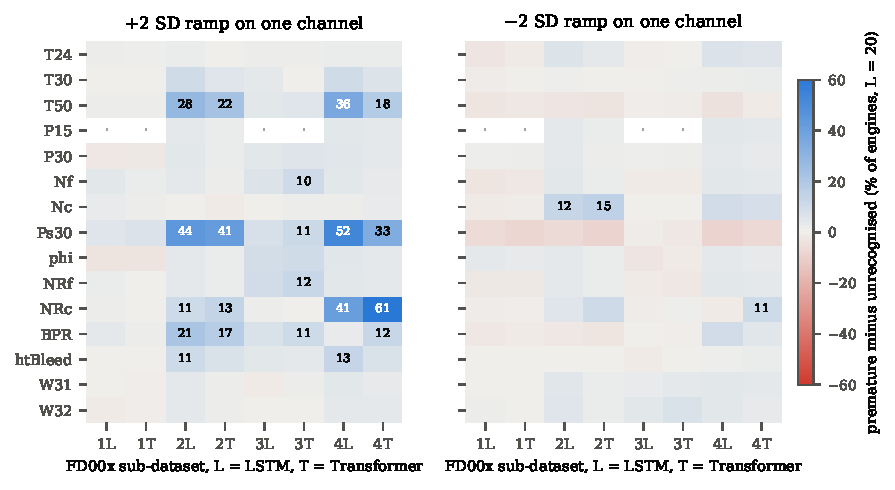
\includegraphics[width=\textwidth]{figures/fig3.pdf}
\caption{Single-channel ramps of $+2$ SD (left) and $-2$ SD (right) on the final window: premature minus unrecognised rate (\% of evaluated engines, heteroscedastic head, $L=20$); blue: premature side, red: unrecognised side; values of magnitude 10 or more are printed. Dots mark channels not used on single-condition data.}
\label{fig:chan}
\end{figure}

\subsection{Drift along trajectories and first triggers}\label{sec:traj}
Re-zeroing the ramp in every window is not what produces the errors. A drift accumulating at 0.02 SD per cycle along each test trajectory gives terminal-window premature rates of \RVPremRate\% (all channels positive) and \RVPremRateAligned\% (aligned). Evaluating every window of each test trajectory and recording the first trigger (Supplement S11), premature first triggers rise from \RVTrajCleanPrem\% of engines on clean inputs to \RVTrajPosPrem\% under the positive drift and \RVTrajAlignedPrem\% under the aligned drift, with a mean of \RVTrajAlignedForgone{} cycles of remaining life beyond the lead time at the first trigger. Under the anti-aligned drift, the share of engines that reach $y\le L$ inside the recorded trajectory without any trigger rises from \RVTrajCleanMiss\% to \RVTrajAntiMiss\%. Only \RVTrajReach{} engines per test set reach $y\le20$ before their records end, so this miss rate rests on few engines. The terminal-window pattern thus carries over to the first-trigger time, which is what a maintenance planner experiences.

\subsection{Mean or scale}\label{sec:swap}
A contracted scale raises the lower bound, so scale contraction alone cannot trigger earlier. Taking the mean and the scale of the heteroscedastic head separately from the clean or the perturbed condition, the mean alone adds \RVSwapMu{} points of premature triggers at $+2$ SD and \RVSwapMuNeg{} points of unrecognised needs at $-2$ SD; adding the perturbed scale changes them by \RVSwapSg{} and \RVSwapSgNeg{} points. The mean shift is therefore the main driver, and the predicted scale does not widen enough to keep the bound away from the lead time. The range-scale output swaps of the earlier analysis, including per-cell intervals and the additive-noise decomposition, agree (Supplement S5). This is an output-level decomposition, not a physical mechanism.

\subsection{Sensitivity of the decision findings}\label{sec:sens}
Varying the bound level ($\alpha=0.10,0.05,0.01$), the tolerance band ($\tau=10,20,40$) and the lead time ($L=10,20,30$) leaves the side of the error unchanged in \RVSensAllOK{} \RVSensDir{} mechanism--cell combinations per setting: under $+2$ SD premature triggers exceed unrecognised needs, and under $-2$ SD the reverse (Supplement S10). The premature rate at $+2$ SD and $L=20$ spans \RVSensPremRange\% over these settings, \RVSensPremTolForty\% with the widest tolerance band and \RVSensPremAlphaOne\% at the 99\% bound; the unrecognised rate at $-2$ SD spans \RVSensLateRange\%. A 99\% bound, close to the replacement point found optimal by Mitici et al.,\cite{mitici2023} therefore does not protect against the premature side and only marginally reduces the late side.

The ranking of mechanisms by the binary cost depends on the cost ratio. Over \RVRankGroups{} backbone--sub-dataset--lead-time--condition groups (clean, $+1$ SD ramp, $\pm2$ SD offset, three-channel ramp) at $\alpha=0.05$, $\tau=20$, the full ranking changes between cost ratios 5, 20 and 100 in \RVRankChg{} and the top mechanism in \RVTopChg; choosing the mechanism under the wrong ratio costs more than 10\% above the best mechanism at the true ratio in \RVRegretTen{} groups. Across bound levels and bands the counts are \RVRankChgRange, \RVTopChgRange{} and \RVRegretTenRange. A mechanism can be chosen once the cost ratio is fixed; the choice is not portable across ratios.

\section{Discussion}
\subsection{What the results change in evaluation practice}
Four practices follow, within the conditions tested. First, an interval that feeds a lower-bound maintenance rule should be evaluated through the rule, with both trigger errors reported beside coverage and with engine-level intervals. A central coverage near nominal did not certify the one-sided bound on clean data, and under degradation the one-sided coverage was near perfect exactly when premature triggers were most frequent. Second, robustness tests should vary the alignment of a shift with the degradation signature and its channel set, not only its magnitude, because these set the side of the error. Third, perturbation sizes should be expressed within operating regimes. Set as a share of the training range, the same nominal level was about \RVRatioFactor{} times larger in SD units on the six-condition sub-datasets than on the single-condition ones; in that scale, the earlier analysis (Supplements S3--S5) found far more damage on six-condition data, and at matched SD the contrast disappears: at $+1$ SD, premature rates are \RVPremOneSingle\% on single-condition and \RVPremOneSix\% on six-condition data, and at $+2$ SD \RVPremTwoSingle\% and \RVPremTwoSix\%. Fourth, the share of out-of-range inputs is not a risk indicator for drift: it stayed below \RVFoobTwo\% while premature or unrecognised rates reached their ceilings.

\subsection{What cannot be inferred}
The perturbations are not calibrated to any instrument; whether a 1--2 SD drift over 30 cycles is realistic depends on the sensor and on how quickly drift is detected and corrected in service. A shift aligned with the degradation signature is, within one window, indistinguishable from degradation by construction, so the results do not show that the models misread drift as degradation in any deeper sense; they show what a lower-bound rule does when it receives such inputs. The study does not estimate first-maintenance cost, availability or safety, and the binary loss is not a maintenance-cost model. The trajectory analysis uses truncated test records, in which few engines reach the lead time. The results do not extend to N-CMAPSS or recorded flight data, other backbones, quantile-regression or adaptive conformal intervals, or other rules.

\subsection{Limitations}
The data are simulated, and two backbones with fixed hyperparameters were studied. The five models per backbone use five partitions, so engine-level intervals are conditional on those models, and initialisation and partition variability are confounded. Channel-subset results rest on ten draws per cell and the single-channel results on one ramp size. The degradation-trend signs come from univariate correlations and do not describe the model's multivariate response, which is why single channels can behave against their trend. Calibration-unit alternatives were evaluated for the conformal mechanism only. All analyses were run once after the protocol was fixed, are exploratory and not pre-registered. The literature comparison in Supplement S8 read three studies in full text and the others from their abstracts. Reproducibility is layered: released result files regenerate the earlier tables; the new analyses rerun inference from released checkpoints with the scripts listed in Supplement S7; training is not re-run.

\section{Conclusion}
In this C-MAPSS stress test, the interval metrics that are usually reported did not reveal which maintenance error a degraded sensor would cause. Central coverage fell for shifts in either direction; the one-sided coverage of the lower bound rose to \RVCovTwo{} while \RVPremTwo\% of evaluated engines were triggered prematurely, and fell only when needed maintenance was missed. The side of the error followed whether the shift moved the inputs along or against the degradation signature the model had learned, for all channels, channel subsets and single channels, for ramps within a window and for drifts accumulating along trajectories, and it did not change with the bound level, the tolerance band or the lead time. How large a shift is depends on the reference: as a share of the training range, sizes differed by a factor of about \RVRatioFactor{} between operating regimes. Interval evaluations meant for maintenance should report premature and unrecognised errors separately with engine-level uncertainty, test shifts with different alignments and channel sets, and scale them within operating regimes. Whether the same holds on recorded data and for other rules remains open.

\section*{Statements and Declarations}
\noindent\textbf{Ethical considerations.} Not applicable; the study uses a public simulated dataset and involves no human or animal subjects.\\[2pt]
\noindent\textbf{Declaration of conflicting interest.} The author declared no potential conflicts of interest with respect to the research, authorship and/or publication of this article.\\[2pt]
\noindent\textbf{Funding statement.} The author received no financial support for the research, authorship and/or publication of this article.\\[2pt]
\noindent\textbf{Declaration of generative AI use.} The AI assistant Claude (Anthropic) was used to help write and run the analysis code, to restructure and edit the text, and to check numbers and cross-references against result files. The author designed the study, reviewed and verified all outputs, and takes full responsibility for the content of the article. No AI tool is listed as an author.\\[2pt]
\noindent\textbf{Data availability.} The C-MAPSS data are available from the NASA Prognostics Center of Excellence. Code, trained checkpoints, result files and the scripts that generate the tables and numbers of this paper are in the public repository \ifanon given to the editor\else\url{https://github.com/jeff-1980/paper2-JRR}\fi. Training is not re-run by these scripts.

\begin{thebibliography}{99}
\small
\setlength{\itemsep}{0pt}
\bibitem{kamariotis2024} Kamariotis A, Tatsis K, Chatzi E, Goebel K, Straub D. A metric for assessing and optimizing data-driven prognostic algorithms for predictive maintenance. Reliab Eng Syst Saf 2024; 242: 109723. DOI: 10.1016/j.ress.2023.109723.
\bibitem{mitici2023} Mitici M, de Pater I, Barros A, Zeng Z. Dynamic predictive maintenance for multiple components using data-driven probabilistic RUL prognostics: the case of turbofan engines. Reliab Eng Syst Saf 2023; 234: 109199. DOI: 10.1016/j.ress.2023.109199.
\bibitem{depater2022} de Pater I, Reijns A, Mitici M. Alarm-based predictive maintenance scheduling for aircraft engines with imperfect Remaining Useful Life prognostics. Reliab Eng Syst Saf 2022; 221: 108341. DOI: 10.1016/j.ress.2022.108341.
\bibitem{lee2022} Lee J, Mitici M. Deep reinforcement learning for predictive aircraft maintenance using probabilistic Remaining-Useful-Life prognostics. Reliab Eng Syst Saf 2023; 230: 108908. DOI: 10.1016/j.ress.2022.108908.
\bibitem{basora2025} Basora L, Viens A, Arias Chao M, Olive X. A benchmark on uncertainty quantification for deep learning prognostics. Reliab Eng Syst Saf 2025; 253: 110513. DOI: 10.1016/j.ress.2024.110513.
\bibitem{piao2025} Piao S, Huang R, Tsung F. CRULP: Reliable RUL Estimation Inspired by Conformal Prediction. IEEE Trans Instrum Meas 2025; 74: 1--11. DOI: 10.1109/tim.2024.3522678.
\bibitem{xu2026} Xu W, Gao S, Wang Z, Zio E. A novel uncertainty-aware framework for remaining useful life prediction integrating uncertainty quantification and calibration. Reliab Eng Syst Saf 2026; 275: 112763. DOI: 10.1016/j.ress.2026.112763.
\bibitem{javanmardi2022} Javanmardi A, H\"ullermeier E. Conformal prediction intervals for remaining useful lifetime estimation. arXiv 2022; 2212.14612. DOI: 10.48550/arXiv.2212.14612.
\bibitem{hachem2024} Hachem H, Vu HC, Fouladirad M. Different methods for RUL prediction considering sensor degradation. Reliab Eng Syst Saf 2024; 243: 109897. DOI: 10.1016/j.ress.2023.109897.
\bibitem{xu2023} Li X, Xu Y, Li N, Yang B, Lei Y. Remaining Useful Life Prediction With Partial Sensor Malfunctions Using Deep Adversarial Networks. IEEE/CAA J Autom Sinica 2023; 10(1): 121--134. DOI: 10.1109/jas.2022.105935.
\bibitem{tang2026} Tang D. A deep learning framework for remaining useful life prediction of turbofan engines with partial sensor failure. PLoS One 2026; 21(4): e0347312. DOI: 10.1371/journal.pone.0347312.
\bibitem{saxena2008} Saxena A, Goebel K, Simon D, Eklund N. Damage propagation modeling for aircraft engine run-to-failure simulation. Proc 1st Int Conf Prognostics Health Manag (PHM) 2008: 1--9.
\bibitem{nix1994} Nix DA, Weigend AS. Estimating the mean and variance of the target probability distribution. Proc IEEE Int Conf Neural Networks (ICNN) 1994: 55--60. DOI: 10.1109/ICNN.1994.374138.
\bibitem{gal2016} Gal Y, Ghahramani Z. Dropout as a Bayesian approximation: representing model uncertainty in deep learning. Proc Int Conf Mach Learn (ICML) 2016; 48: 1050--1059.
\bibitem{kendall2017} Kendall A, Gal Y. What uncertainties do we need in Bayesian deep learning for computer vision? Adv Neural Inf Process Syst 2017; 30.
\bibitem{lakshminarayanan2017} Lakshminarayanan B, Pritzel A, Blundell C. Simple and scalable predictive uncertainty estimation using deep ensembles. Adv Neural Inf Process Syst 2017; 30.
\bibitem{barber2023} Barber RF, Cand\`es EJ, Ramdas A, Tibshirani RJ. Conformal prediction beyond exchangeability. Ann Stat 2023; 51: 816--845.
\end{thebibliography}

\end{document}
